\documentclass{article}

% if you need to pass options to natbib, use, e.g.:
%     \PassOptionsToPackage{numbers, compress}{natbib}
% before loading neurips_2026
\PassOptionsToPackage{numbers,sort&compress}{natbib}
% The authors should use one of these tracks.
% Before accepting by the NeurIPS conference, select one of the options below.
% 0. "default" for submission
\usepackage[main, preprint]{neurips_2026}
% the "default" option is equal to the "main" option, which is used for the Main Track with double-blind reviewing.
% 1. "main" option is used for the Main Track
%  \usepackage[main]{neurips_2026}
% 2. "position" option is used for the Position Paper Track
%  \usepackage[position]{neurips_2026}
% 3. "eandd" option is used for the Evaluations & Datasets Track
 % \usepackage[eandd]{neurips_2026}
 % if you need to opt-in for a single-blind submission in the E&D track:
 %\usepackage[eandd, nonanonymous]{neurips_2026}
% 4. "creativeai" option is used for the Creative AI Track
%  \usepackage[creativeai]{neurips_2026}
% 5. "sglblindworkshop" option is used for the Workshop with single-blind reviewing
 % \usepackage[sglblindworkshop]{neurips_2026}
% 6. "dblblindworkshop" option is used for the Workshop with double-blind reviewing
%  \usepackage[dblblindworkshop]{neurips_2026}

% After being accepted, the authors should add "final" behind the track to compile a camera-ready version.
% 1. Main Track
 % \usepackage[main, final]{neurips_2026}
% 2. Position Paper Track
%  \usepackage[position, final]{neurips_2026}
% 3. Evaluations & Datasets Track
 % \usepackage[eandd, final]{neurips_2026}
% 4. Creative AI Track
%  \usepackage[creativeai, final]{neurips_2026}
% 5. Workshop with single-blind reviewing
%  \usepackage[sglblindworkshop, final]{neurips_2026}
% 6. Workshop with double-blind reviewing
%  \usepackage[dblblindworkshop, final]{neurips_2026}
% Note. For the workshop paper template, both \title{} and \workshoptitle{} are required, with the former indicating the paper title shown in the title and the latter indicating the workshop title displayed in the footnote.
% For workshops (5., 6.), the authors should add the name of the workshop, "\workshoptitle" command is used to set the workshop title.
% \workshoptitle{WORKSHOP TITLE}

% "preprint" option is used for arXiv or other preprint submissions
 % \usepackage[preprint]{neurips_2026}

% to avoid loading the natbib package, add option nonatbib:
%    \usepackage[nonatbib]{neurips_2026}

\usepackage[utf8]{inputenc} % allow utf-8 input
\usepackage[T1]{fontenc}    % use 8-bit T1 fonts
\usepackage{url}            % simple URL typesetting
\usepackage{booktabs}       % professional-quality tables
\usepackage{amsfonts}       % blackboard math symbols
\usepackage{nicefrac}       % compact symbols for 1/2, etc.
\usepackage{microtype}      % microtypography
\usepackage{xcolor}         % colors
\usepackage{graphicx}
\usepackage{amsmath}
\usepackage{longtable}
\usepackage{bbm}
% \usepackage{caption} % preamble에 없으면 추가
\definecolor{rliableolive}{HTML}{DCE6F0}
\usepackage[most]{tcolorbox}
\usepackage{wrapfig}
\usepackage{enumitem}
\usepackage{makecell}
\usepackage{tabularx} % preamble
\usepackage{subcaption}
\usepackage{hyperref}       % hyperlinks
\usepackage{pifont}          % \cmark / \xmark
\usepackage[table]{xcolor}


\newcommand{\cmark}{\textcolor{green!60!black}{\ding{51}}}
\newcommand{\xmark}{\textcolor{red!70!black}{\ding{55}}}
\tcbset{
  aibox/.style={
    width=\linewidth,
    top=4pt,
    bottom=4pt,
    colback=rliableolive!8!white,
    colframe=black,
    colbacktitle=black,
    enhanced,
    center,
    attach boxed title to top left={yshift=-0.1in,xshift=0.15in},
    boxed title style={boxrule=0pt,colframe=white,},
  }
}
\newcommand{\method}{\emph{v}OPD}
\newtcolorbox{AIbox}[2][]{aibox,title=#2,#1} %for the box
% Note. For the workshop paper template, both \title{} and \workshoptitle{} are required, with the former indicating the paper title shown in the title and the latter indicating the workshop title displayed in the footnote. 
\title{KL for a KL: On-Policy Distillation with Control Variate Baseline}
% The \author macro works with any number of authors. There are two commands
% used to separate the names and addresses of multiple authors: \And and \AND.
%
% Using \And between authors leaves it to LaTeX to determine where to break the
% lines. Using \AND forces a line break at that point. So, if LaTeX puts 3 of 4
% authors names on the first line, and the last on the second line, try using
% \AND instead of \And before the third author name.

% \author{%
%   Minjae Oh, Sangjun Song, Gyubin Choi, Yunho Choi, Yohan Jo\thanks{Corresponding Author} \\
%   Graduate School of Data Science, Seoul National University \\
%   \texttt{\{kosair, ssangjun706, yeppi315, yohan.jo\}@snu.ac.kr} \\
%   % examples of more authors
%   % \And
%   % Coauthor \\
%   % Affiliation \\
%   % Address \\
%   % \texttt{email} \\
%   % \AND
%   % Coauthor \\
%   % Affiliation \\
%   % Address \\
%   % \texttt{email} \\
%   % \And
%   % Coauthor \\
%   % Affiliation \\
%   % Address \\
%   % \texttt{email} \\
%   % \And
%   % Coauthor \\
%   % Affiliation \\
%   % Address \\
%   % \texttt{email} \\
% }

\author{%
  Minjae Oh \\
  Graduate School of Data Science \\
  Seoul National University \\
  \texttt{kosair@snu.ac.kr} \\
  \And
  Sangjun Song \\
  Graduate School of Data Science \\
  Seoul National University \\
  \texttt{ssangjun706@snu.ac.kr} \\
  \AND
  Gyubin Choi \\
  Graduate School of Data Science \\
  Seoul National University \\
  \texttt{yeppi315@snu.ac.kr} \\
  \And
  Yunho Choi \\
  Graduate School of Data Science \\
  Seoul National University \\
  \texttt{dbsgh7177@snu.ac.kr} \\
  \AND
  Yohan Jo$^\dagger$ \\
  Graduate School of Data Science \\
  Seoul National University \\
  \texttt{yohan.jo@snu.ac.kr} \\
}
\begin{document}
\maketitle
\begin{abstract}
On-Policy Distillation (OPD) has emerged as a dominant post-training paradigm for large language models, especially for reasoning domains. However, OPD remains unstable in practice due to the high gradient variance of its single-sample Monte Carlo estimator, and recipes for stable training are still immature. We propose \method{} (\textbf{O}n-\textbf{P}olicy \textbf{D}istillation with a control \emph{\textbf{v}}ariate baseline), which casts OPD as policy-gradient RL and stabilizes it by introducing a control variate baseline—canonically a value function—from the RL literature. We show that the OPD value function admits a closed form as the per-token negative reverse KL divergence between the student and the teacher, available directly from the already-computed forward pass with no additional critic or inference. Existing stabilization methods either compute the full token-level reverse KL over the entire vocabulary, adding significant overhead, or restrict it to a top-$k$ support, biasing the objective. \method{} instead preserves the lightweight single-sample estimator, subtracting the value function as a detached baseline to keep the gradient unbiased while reducing variance. Furthermore, we show that a top-$k$ approximation of the baseline further lowers cost without compromising performance.  Across mathematical and scientific reasoning benchmarks, \method{} consistently outperforms vanilla OPD and matches the most expensive full-vocabulary baseline, offering an efficient stabilization of On-Policy Distillation through principled RL variance reduction.\footnote{Code is available at \url{https://github.com/holi-lab/vOPD}.}
\end{abstract}

\def\thefootnote{\fnsymbol{footnote}}
\footnotetext[2]{Corresponding author.}
\def\thefootnote{\arabic{footnote}}

\section{Introduction}
Large Language Models have made remarkable advances in reasoning, accompanied by improvements in post-training recipes~\citep{jaech2024openai, yang2025qwen3, team2025kimi}. A key factor has been Reinforcement Learning with Verifiable Rewards (RLVR)~\citep{lambert2024tulu, guo2025deepseek}, which trains LLMs directly against easily verifiable rewards---answer correctness, code execution---sidestepping the noise and reward hacking introduced by learned reward models. RLVR has been successful thanks to its simple recipe, but this simplicity comes at a cost: LLMs generate thousands of intermediate tokens during reasoning before receiving a single scalar reward for the final answer. RLVR methods must perform credit assignment over long chains of thought from a single sparse scalar signal. This sparse supervision demands large rollouts and prolonged training, making training progress painfully slow.

On-Policy Distillation (OPD)~\citep{gu2024minillm, agarwal2024onpolicy} has emerged as an attractive alternative to RLVR when a strong teacher is available. Rather than relying on a sparse terminal reward, OPD minimizes the reverse KL divergence between the student and the teacher via dense, token-level signals, enabling faster training~\citep{lightman2024let}. Because it is on-policy and reward-driven, OPD can naturally be implemented using standard RL pipelines with a single-sample Monte Carlo estimator~\citep{lu2025onpolicydistillation}, and empirically matches RLVR accuracy with a fraction of the compute~\citep{patino2025opd}. Its effectiveness has been demonstrated in industrial-level post-training such as Qwen3, GLM-5, Nemotron-Cascade2, and DeepSeek-V4~\citep{yang2025qwen3, zeng2026glm, yang2026nemotron2, deepseekai2026deepseekv4}. Despite this success, OPD's optimization recipe remains underdeveloped: training is unstable in practice, and stabilization techniques are still immature relative to the recipes that drive successful RLVR training~\citep{yu2025dapo, khatri2025art, zheng2025gspo, chen2025minimax, liu2026tricks}. The most widely adopted fix replaces the single-sample estimator with a full-vocabulary token-level KL, incurring additional compute overhead~\citep{agarwal2024onpolicy}; a lighter-weight variant restricts the KL to a top-$k$ support, which biases the gradient away from the true objective and still adds compute, yet yields only marginal gains~\citep{li2026rethinkingopd}. In contrast, we turn to the RL interpretation of OPD and propose a principled, low-compute method that controls variance while preserving the efficient single-sample Monte Carlo estimator.

We propose \textbf{\method{}} (\textbf{O}n-\textbf{P}olicy \textbf{D}istillation with a control \emph{\textbf{v}}ariate baseline), which leverages a standard tool from policy-gradient RL to reduce gradient variance: subtracting a control variate baseline~\citep{williams1992simple, sutton1999policygrad, greensmith2004variance}. Baseline subtraction for variance reduction underlies actor-critic methods such as PPO, and more recently GRPO and RLOO~\citep{schulman2017ppo, mnih2016asynchronous, ahmadian2024back, shao2024deepseekmath} (see \S~\ref{sec:vopd_value}). \method{} reduces variance without biasing the gradient in expectation. The standard choice of baseline is the value function, and we show that for OPD this quantity admits a computable closed form: the per-token negative reverse KL between the student and the teacher at each token. The baseline is therefore available from the same forward pass that already computes the OPD objective---without an additional critic model, extra rollouts, or additional backward passes. We show that the baseline can be approximated using only the top-$k$ student tokens at a lower cost; crucially, because this approximation does not depend on the sampled token, it preserves the unbiasedness of the gradient regardless of $k$ (see \S~\ref{sec:vopd-topk}). Furthermore, we find empirically that the choice of $k$ has little effect on performance (see \S~\ref{sec:exp_ablation}).

We evaluate \method{} on four models from the Qwen3~\citep{yang2025qwen3} and Olmo-3~\citep{olmo2025olmo} families across six reasoning benchmarks spanning mathematics and science---MATH500~\citep{hendrycks2021math,lightman2024let}, Minerva Math~\citep{lewkowycz2022solving}, AMC23~\citep{maa_amc}, AIME24/25~\citep{maa_aime}, SciKnowEval~\citep{feng2024sciknoweval}, and GPQA-Diamond~\citep{rein2024gpqa}---demonstrating consistent improvements over baseline methods. \method{} delivers an absolute average accuracy gain of up to +3\%  on average over base OPD, with improvements of up to +6.2\% on MATH500 (see \S\S~\ref{sec:exp-math}~and~\ref{sec:exp-sci}). Against the two stabilization variants, \method{} substantially outperforms top-$k$ OPD and matches full-vocabulary OPD while reducing wall-clock time up to 57.7\%. We further validate the stability of \method{} through consistently lower gradient norms, and show that it acts as a regularizer on destabilizing reward tokens (see \S~\ref{sec:exp-further}). Overall, \method{} bridges RL and knowledge distillation, providing a principled, efficient approach to stable On-Policy Distillation.

\section{Preliminaries}
\label{sec:prelim}
\subsection{On-Policy Distillation}
\label{sec:opd}
On-Policy Distillation (OPD)~\citep{agarwal2024onpolicy,gu2024minillm} trains the student by minimizing the reverse KL divergence between the student ($\pi_\theta$) and the teacher ($\pi_T$):
\begin{equation}
\label{eq:RKL}
\mathbb{D}_\mathrm{KL}\!\left(\pi_\theta \,\|\, \pi_T\right)
\;=\;
\mathbb{E}_{x\sim \mathcal{D},\, y\sim \pi_\theta(\cdot\mid x)}
\!\left[\log \frac{\pi_\theta(y\mid x)}{\pi_T(y\mid x)}\right],
\end{equation}
where $x$ is a prompt drawn from a dataset $\mathcal{D}$ and $y = (y_1, \ldots, y_{|y|})$ is a response of length $|y|$. Importantly, OPD samples from the student during generation to obtain an unbiased estimator of the KL.  On-policy learning mitigates exposure bias~\citep{ranzato2015exposurebias}---the train-test discrepancy in off-policy training, where the model is trained on static data but conditions on its own outputs at test time. This has enabled effective training on long Chain-of-Thought reasoning tasks such as mathematics~\citep{wei2022chain,yang2025qwen3,lu2025onpolicydistillation}. In practice, Eq.~\eqref{eq:RKL} is commonly optimized via a single-sample Monte Carlo estimate, by maximizing the following token-level objective, where $c_t = (x, y_{<t})$ denotes the context at step $t$~\citep{lu2025onpolicydistillation}:
\begin{equation}
\label{eq:opd-objective}
\mathcal{J}_\text{OPD}(\theta)
\;=\;
\mathbb{E}_{x\sim\mathcal{D},\, y \sim \pi_\theta(\cdot\mid x)}
\!\left[\sum_{t=1}^{|y|} \log \frac{\pi_T(y_t \mid c_t)}{\pi_\theta(y_t \mid c_t)}\right].
\end{equation}
Following recent practice~\citep{lu2025onpolicydistillation, zeng2026glm, ko2026scaling}, Eq.~\eqref{eq:opd-objective} is optimized as policy-gradient 
RL~\citep{williams1992simple, sutton1999policygrad} by defining the per-token 
reward $r_t(c_t, y_t) = \log \pi_T(y_t \mid c_t) - \log \pi_\theta(y_t \mid c_t)$  as a fixed scalar with no gradient flowing through it. This yields the gradient:
\begin{equation}
\label{eq:opd-gradient}
\nabla_\theta \mathcal{J}_\text{OPD}(\theta)
\;=\;
\mathbb{E}_{x\sim\mathcal{D},\, y\sim \pi_\theta(\cdot\mid x)}
\!\left[\sum_{t=1}^{|y|}
\underbrace{\bigl(\log \pi_T(y_t \mid c_t) - \log \pi_\theta(y_t \mid c_t)\bigr)}_{\textstyle r_t(c_t,y_t)}
\,\nabla_\theta \log \pi_\theta(y_t \mid c_t)\right].
\end{equation}
We refer to this base formulation as \textbf{OPD} throughout the paper. Its backward pass touches only $\nabla_\theta\log \pi_\theta(y_t\mid c_t)$ at the single sampled token, making it the most computationally efficient variant. However, the single-sample Monte Carlo estimator carries high variance, leading to training instability. We next discuss two variants that aim to stabilize OPD, along with the drawbacks of each.

\paragraph{Full-vocabulary OPD ($\text{OPD}_\text{full-V}$).}
To mitigate the variance of the single-sample estimator, one variant
computes the full per-token KL over the entire vocabulary $\mathcal{V}$~\citep{agarwal2024onpolicy}:
\begin{equation}
\label{eq:opd-full-J}
\mathcal{J}_{\text{OPD}_\text{full-V}}(\theta)
\;=\;
-\,\mathbb{E}\!\left[\, \sum_{t=1}^{|y|} \mathbb{D}_\mathrm{KL}\!\bigl(\pi_\theta(\cdot\mid c_t) \,\big\|\, \pi_T(\cdot\mid c_t)\bigr) \,\right]
\;=\;
\mathbb{E}\!\left[\, \sum_{t=1}^{|y|} \sum_{v \in \mathcal{V}} \pi_\theta(v\mid c_t)\,r_t(c_t,v) \,\right],
\end{equation}
where $r_t(c_t,v) = \log\pi_T(v\mid c_t) - \log\pi_\theta(v\mid c_t)$ extends
the per-token reward to any vocabulary entry. Similar to Eq.~\eqref{eq:opd-gradient}, Eq.~\eqref{eq:opd-full-J} can be optimized by the corresponding gradient:
\begin{equation}
\label{eq:opd-full-grad}
\nabla_\theta\mathcal{J}_{\text{OPD}_\text{full-V}}(\theta)
\;=\;
\mathbb{E}\!\left[\, \sum_{t=1}^{|y|} \sum_{v \in \mathcal{V}} \pi_\theta(v\mid c_t)\,r_t(c_t,v)\,\nabla_\theta\log \pi_\theta(v\mid c_t) \,\right],
\end{equation}
which is the exact expectation of Eq.~\eqref{eq:opd-gradient} under $v \sim \pi_\theta$, and is therefore zero-variance for a given $c_t$. The cost, however, is substantial as it requires a backward pass against the full vocabulary at every token (e.g., $|\mathcal{V}| \approx 150\mathrm{k}$ for Qwen3~\citep{yang2025qwen3}).

\paragraph{Top-$k$ OPD ($\text{OPD}_\text{top-$k$}$).}
A lightweight variant of $\text{OPD}_\text{full-V}$ computes the per-token KL against only the top-$k$ tokens, with $k \ll |\mathcal{V}|$~\citep{li2026rethinkingopd}. We consider the student top-$k$ version, restricting the KL to the support $S_t$ of the student's $k$ most likely tokens:
\begin{equation}
\label{eq:opd-topk-J}
\mathcal{J}_{\text{OPD}_\text{top-$k$}}(\theta)
\;=\;
-\,\mathbb{E}\!\left[\, \sum_{t=1}^{|y|} \mathbb{D}_\mathrm{KL}\!\bigl(\bar\pi_\theta(\cdot\mid c_t) \,\big\|\, \bar\pi_T(\cdot\mid c_t)\bigr) \,\right],
\quad
\bar\pi(v\mid c_t) = \frac{\pi(v\mid c_t)\,\mathbf{1}[v \in S_t]}{\sum_{u \in S_t} \pi(u\mid c_t)}.
\end{equation}
Eq.~\eqref{eq:opd-topk-J} is optimized by a gradient of the same shape as Eq.~\eqref{eq:opd-full-grad}, but restricted to $S_t$ and acting on the renormalized distributions:
\begin{equation}
\label{eq:opd-topk-grad}
\nabla_\theta\mathcal{J}_{\text{OPD}_\text{top-$k$}}(\theta)
\;=\;
\mathbb{E}\!\left[\, \sum_{t=1}^{|y|} \sum_{v \in S_t}
\bar\pi_\theta(v\mid c_t)\,\log\frac{\bar\pi_T(v\mid c_t)}{\bar\pi_\theta(v\mid c_t)}
\nabla_\theta\log \bar\pi_\theta(v\mid c_t) \,\right].
\end{equation}
The backward pass now flows through $k$ tokens per position, rather than the single sampled token in OPD---substantially more lightweight than the full vocabulary, but heavier than base OPD. More importantly, this comes at the cost of \emph{bias}: $\nabla_\theta\mathcal{J}_{\text{OPD}_\text{top-$k$}} \neq \nabla_\theta\mathcal{J}_\text{OPD}$, since restricting to $S_t$ omits out-of-support mass. In practice, despite this added compute, $\text{OPD}_\text{top-$k$}$ has been reported to yield only marginal gains over base OPD~\citep{li2026rethinkingopd}, an observation we confirm in \S~\ref{sec:exp-math}.

\subsection{Control Variate Baseline in Reinforcement Learning}
\label{sec:baseline}
As OPD in Eq.~\eqref{eq:opd-gradient} is a form of RL, we now introduce the standard variance-reduction tool used in policy-gradient RL: subtracting a baseline $b_t(c_t)$ from the per-step reward, yielding the \emph{advantage} $a_t(c_t,y_t) = r_t(c_t,y_t) - b_t(c_t)$~\citep{williams1992simple,sutton1999policygrad}:
\begin{equation}
\label{eq:baseline-grad}
\nabla_\theta \mathcal{J}(\theta)
\;=\;
\mathbb{E}\!\left[\, \sum_{t=1}^{|y|} \bigl(r_t(c_t,y_t) - b_t(c_t)\bigr)\,\nabla_\theta\log \pi_\theta(y_t\mid c_t) \,\right].
\end{equation}
This has two properties that make it successful in modern RL. \textbf{(i)~Unbiasedness:} for \emph{any} $b_t$ that is independent of the sampled action $y_t$, $\mathbb{E}[b_t(c_t)\nabla_\theta\log\pi_\theta(y_t\mid c_t)] = 0$, so the expected gradient is unchanged, and the loss remains unbiased (see \S~\ref{app:unbiased}). \textbf{(ii)~Variance reduction:} a well-defined baseline reduces the gradient variance, the canonical choice being the value function $V^{\pi_\theta}(c_t) = \mathbb{E}_{y_t \sim \pi_\theta(\cdot\mid c_t)}[r_t(c_t,y_t)]$ (see \S~\ref{app:variance}). Baseline subtraction underlies the success of essentially every modern policy-gradient algorithm, from classical actor-critic methods with a learned value baseline~\citep{mnih2016asynchronous, schulman2017ppo,schulman2016high} to the group-relative baseline in GRPO~\citep{shao2024deepseekmath}.

\section{Control Variate Baseline for OPD}
\label{sec:method}
We introduce \method{} (\textbf{O}n-\textbf{P}olicy \textbf{D}istillation with a control \emph{\textbf{v}}ariate baseline), which addresses the high variance of OPD (\S~\ref{sec:opd}) by exploiting its RL interpretation and subtracting a control variate baseline (\S~\ref{sec:baseline}). \method{} is an unbiased, lower-variance version of OPD that requires no additional backward passes, making it computationally efficient. We first show that the value function of OPD is available in closed form as the per-step reverse KL, and discuss the loss formulation of \method{} (see \S~\ref{sec:vopd_value}). We then propose an even more computationally efficient version using a top-$k$ KL estimate (see \S~\ref{sec:vopd-topk}), and compare our methods with the various variants of OPD (see \S~\ref{sec:opd-comparison}).

\subsection{The Value Function of OPD}
\label{sec:vopd_value}
As discussed in \S~\ref{sec:baseline}, the standard choice of baseline is the value function. Recall the OPD per-token reward $r_t(c_t, y_t) = \log \pi_T(y_t\mid c_t) - \log \pi_\theta(y_t\mid c_t)$ from Eq.~\eqref{eq:opd-gradient}. By definition, taking the expectation of $r_t$ under the student distribution ($\pi_\theta$) gives the per-step value function:
\begin{equation}
\label{eq:value-fn}
V^{\pi_\theta}(c_t)
\;=\;
\mathbb{E}_{y_t \sim \pi_\theta(\cdot\mid c_t)}[r_t(c_t, y_t)]
\;=\;
-\,\mathbb{D}_\mathrm{KL}\!\bigl(\pi_\theta(\cdot\mid c_t) \,\big\|\, \pi_T(\cdot\mid c_t)\bigr).
\end{equation}
The value function is exactly the negative per-step reverse KL~\citep{tang2025few}, computable in closed form using the already-computed student ($\pi_\theta$) and teacher ($\pi_T$) distributions at context $c_t$ without a learned value network or an additional forward pass. Substituting Eq.~\eqref{eq:value-fn} as the baseline in Eq.~\eqref{eq:baseline-grad} gives the \method{} gradient estimator with advantage $a_t(c_t, y_t)$:
\begin{equation}
\label{eq:vopd-full-grad}
\nabla_\theta \mathcal{J}_{\text{\method{}}}(\theta)
\;=\;
\mathbb{E}\!\left[\, \sum_{t=1}^{|y|}
\underbrace{\Bigl( r_t(c_t, y_t) + \mathbb{D}_\mathrm{KL}\!\bigl(\pi_\theta(\cdot\mid c_t) \,\big\|\, \pi_T(\cdot\mid c_t)\bigr) \Bigr)}_{\textstyle a_t(c_t,y_t)}
\,\nabla_\theta \log \pi_\theta(y_t\mid c_t) \,\right],
\end{equation}
which is denoted by \method$_{\text{full-V}}$; the subscript indicates the expectation over the full vocabulary to compute the KL baseline. As discussed in \S~\ref{sec:baseline}, this estimator has the same expected gradient as OPD: $\mathbb{E}[\nabla \mathcal{J}_{\text{\method}_{\text{full-V}}}] = \mathbb{E}[\nabla \mathcal{J}_\text{OPD}]$. Importantly, the baseline KL is computed only in the forward pass and does not propagate gradients through the vocabulary, so the backward pass flows only through $\nabla_\theta \log \pi_\theta(y_t\mid c_t)$ at the single sampled token, identical to base OPD.

\paragraph{Variance reduction.}
We now examine where and why \method{} reduces variance, showing it dampens gradients most strongly on the most destabilizing cases. Recent works have identified \emph{high-mismatch tokens}---where the student and the teacher distributions strongly disagree---as the dominant source of OPD's gradient instability: at these tokens, the per-token reward ($r_t$) takes large negative values, producing heavy-tailed gradients that dominate training~\citep{ko2026scaling, li2026rethinkingopd}. \method{}'s baseline directly counteracts this. Since $-V^{\pi_\theta}(c_t) = \mathbb{D}_\mathrm{KL}(\pi_\theta\|\pi_T)$ becomes a large positive value precisely when the student and the teacher strongly disagree, the \method{} advantage $(a_t=r_t+\mathbb{D}_\mathrm{KL}(\pi_\theta\|\pi_T))$ stays bounded even on such heavy-tailed tokens, acting as a regularizer. This token-level reward damping translates directly into a reduction in gradient variance. We show that the per-token variance reduction of \method{} is approximately:
\begin{equation}
\label{eq:variance-reduction}
\underbrace{\mathrm{tr}\!\bigl(\mathrm{Var}[g_\text{OPD}]\bigr)}_{\text{OPD variance}}
\;-\;
\underbrace{\mathrm{tr}\!\bigl(\mathrm{Var}[g_{\text{\method}_{\text{full-V}}}]\bigr)}_{\text{\method{} variance}}
\;\approx\;
\mathbb{D}_\mathrm{KL}\!\bigl(\pi_\theta(\cdot\mid c_t) \,\big\|\, \pi_T(\cdot\mid c_t)\bigr)^{\!2}
\;\cdot\;
\mathbb{E}_{\pi_\theta}\!\bigl[\,\|\nabla_\theta \log \pi_\theta(y_t\mid c_t)\|^2\,\bigr],
\end{equation}
where $g_\text{OPD}$ and $g_{\text{\method}_{\text{full-V}}}$ are the per-step gradient estimators of OPD (Eq.~\eqref{eq:opd-gradient}) and \method$_{\text{full-V}}$ (Eq.~\eqref{eq:vopd-full-grad}), and $\mathrm{tr}(\cdot)$ denotes the matrix trace. We provide a detailed derivation in \S~\ref{app:variance-derivation}. From Eq.~\eqref{eq:variance-reduction}, the variance reduction is largest when the squared $\mathbb{D}_\mathrm{KL}(\pi_\theta\|\pi_T)$ is large at the high-mismatch tokens, which matches our token-level reward damping view. Overall, \method{} dampens the noisy negative long-tail gradients destabilizing OPD, which we further validate empirically in \S~\ref{sec:exp-further}.

\paragraph{Connection to $\text{OPD}_\text{full-V}$.}
A natural question is whether the same baseline could also help $\text{OPD}_\text{full-V}$. The answer is no, and the reason illuminates the relationship between the two methods. Subtracting the value baseline from the $\text{OPD}_\text{full-V}$ gradient (Eq.~\eqref{eq:opd-full-grad}) gives
\begin{equation}
\label{eq:full-v-with-baseline}
\nabla_\theta \mathcal{J}_{\text{OPD}_\text{full-V}}^{\text{+baseline}}
\;=\;
\mathbb{E}\!\left[\, \sum_{t=1}^{|y|} \sum_{v \in \mathcal{V}}
\pi_\theta(v\mid c_t)\,
\underbrace{\bigl(r_t(c_t,v) - V^{\pi_\theta}(c_t)\bigr)}_{\textstyle a_t(c_t,v)}
\,\nabla_\theta\log \pi_\theta(v\mid c_t) \,\right],
\end{equation}
which is identical to the original gradient because the baseline contribution vanishes:
\begin{equation}
\label{eq:baseline-cancels}
V^{\pi_\theta}(c_t) \sum_{v \in \mathcal{V}} \pi_\theta(v\mid c_t)\,\nabla_\theta\log \pi_\theta(v\mid c_t)
\;=\; V^{\pi_\theta}(c_t)\,\nabla_\theta \!\sum_{v \in \mathcal{V}} \pi_\theta(v\mid c_t) \;=\; 0.
\end{equation}
Because $\text{OPD}_\text{full-V}$ computes the full KL, its gradient already has zero variance at $c_t$, leaving nothing for the baseline to reduce. The baseline becomes useful only once we replace the full-vocabulary expectation with a Monte Carlo estimate, as is done in \method$_\text{full-V}$.

\subsection{Top-$k$ Approximation}
\label{sec:vopd-topk}
While \method$_\text{full-V}$ adds no additional backward-pass cost, it still requires the exact KL computation at $O(|\mathcal{V}|)$ cost. Similar to $\text{OPD}_\text{top-$k$}$ (Eq.~\eqref{eq:opd-topk-J}), we can approximate the baseline KL on the student's top-$k$ support to further reduce compute:
\begin{equation}
\label{eq:vopd-topk-baseline}
\hat b_t(c_t)
\;=\;
-\,\mathbb{D}_\mathrm{KL}\!\bigl(\bar\pi_\theta(\cdot\mid c_t) \,\big\|\, \bar\pi_T(\cdot\mid c_t)\bigr),
\end{equation}
where $\bar\pi$ is the renormalized distribution on the student's top-$k$ support $S_t$ with $k \ll |\mathcal{V}|$. Substituting $\hat b_t$ into Eq.~\eqref{eq:baseline-grad} gives the \method$_\text{top-$k$}$ gradient estimator:
\begin{equation}
\label{eq:vopd-topk-grad}
\nabla_\theta \mathcal{J}_{\text{\method}_\text{top-$k$}}(\theta)
\;=\;
\mathbb{E}\!\left[\, \sum_{t=1}^{|y|}
\underbrace{\Bigl( r_t(c_t,y_t) + \mathbb{D}_\mathrm{KL}\!\bigl(\bar\pi_\theta(\cdot\mid c_t) \,\big\|\, \bar\pi_T(\cdot\mid c_t)\bigr) \Bigr)}_{\textstyle a_t(c_t,y_t)}
\,\nabla_\theta \log \pi_\theta(y_t\mid c_t) \,\right].
\end{equation}

\paragraph{The crucial distinction from $\text{OPD}_\text{top-$k$}$.}
While both methods compute KL with a top-$k$ approximation, they place it in different positions of the estimator. $\text{OPD}_\text{top-$k$}$ uses it as the \emph{loss}, replacing $\mathrm{KL}(\pi_\theta\|\pi_T)$ with $\mathrm{KL}(\bar\pi_\theta\|\bar\pi_T)$, thus changing the optimization target and biasing the gradient. \method$_\text{top-$k$}$ uses it as a \emph{detached baseline} subtracted from the reward. As discussed in \S~\ref{sec:baseline}, because $\hat b_t$ depends only on $\pi_\theta$, $\pi_T$, and $S_t$ but not on the sampled token $y_t$, the gradient remains unbiased. Furthermore, since $\hat b_t$ still approximates the value function $V^{\pi_\theta}(c_t)$, it can still reduce variance. The same approximation in different positions thus has completely different consequences, which we further confirm empirically in \S~\ref{sec:exp-math}: \method$_\text{top-$k$}$ allows substantial gains in practice compared to OPD, while $\text{OPD}_\text{top-$k$}$ does not.

\begin{table}[t]
\centering
\caption{Comparison of OPD variants along key algorithmic axes. Our methods are highlighted.}
\label{tab:method-axes}
\renewcommand{\arraystretch}{1.25}
\begin{tabular}{lccccc}
\toprule
\textbf{Method}
  & \makecell{\textbf{Gradient} \\ \textbf{unbiased?}}
  & \makecell{\textbf{Gradient} \\ \textbf{variance at $\mathbf{c_t}$}}
  & \makecell{\textbf{Backward} \\ \textbf{token count}}
  & \makecell{\textbf{Per-token} \\ \textbf{KL cost}}
  & \makecell{\textbf{Total additional} \\ \textbf{compute}} \\
\midrule
OPD                                         & \cmark & High & 1                 & ---                & None      \\
$\text{OPD}_\text{full-V}$                  & \cmark & None & $|\mathcal{V}|$   & $O(|\mathcal{V}|)$ & High      \\
$\text{OPD}_\text{top-$k$}$                 & \xmark & None & $k$               & $O(k)$             & Medium    \\
\rowcolor{blue!10} \method$_\text{full-V}$  & \cmark & Low  & 1                 & $O(|\mathcal{V}|)$ & Low       \\
\rowcolor{blue!10} \method$_\text{top-$k$}$ & \cmark & Low  & 1                 & $O(k)$             & Very Low  \\
\bottomrule
\end{tabular}
\end{table}
\subsection{Summary: Algorithm Comparison}
\label{sec:opd-comparison}
Table~\ref{tab:method-axes} compares the discussed algorithms along the key axes of bias, variance, and compute. Base OPD is the computationally lightest but suffers from high gradient variance due to its single-sample Monte Carlo estimator. $\text{OPD}_\text{full-V}$ eliminates this variance by computing the per-token KL at $c_t$ over the full vocabulary, but requires $O(|\mathcal{V}|)$ cost for both the per-token KL computation and the backward pass. $\text{OPD}_\text{top-$k$}$ reduces both costs to $O(k)$, but changes the objective by restricting the KL to a truncated support, thereby biasing the gradient. In contrast, \method$_\text{full-V}$ preserves base OPD's unbiased single-token estimator while reducing variance via the value baseline, adding only an additional per-token KL computation in the forward pass. \method$_\text{top-$k$}$ further approximates this baseline on the student's top-$k$ support, preserving unbiasedness while achieving variance reduction at the lowest compute.

\section{Experiments}
\subsection{Experimental Setup}
\label{sec:exp_setup}
\paragraph{Models and methods.} Our primary setting distills Qwen3-1.7B into Qwen3-1.7B-Base~\citep{yang2025qwen3}, mirroring a common industrial OPD configuration where a post-trained checkpoint is distilled back into its base model~\citep{zeng2026glm, yang2026nemotron2, deepseekai2026deepseekv4}. We additionally evaluate three axes: (i) scale, Qwen3-4B into Qwen3-4B-Base; (ii) size mismatch, Qwen3-1.7B into Qwen3-0.6B-Base; and (iii) model family, Olmo-3-7B-Think into Olmo-3-7B-Base~\citep{olmo2025olmo}. We compare \method{} against the three OPD variants from \S~\ref{sec:opd}: base OPD, {OPD}$_\text{full-V}$, and OPD$_\text{top-$k$}$, with both \method{}$_\text{full-V}$ and \method{}$_\text{top-$k$}$. For OPD$_\text{top-$k$}$ we set $k=20$ following~\citet{li2026rethinkingopd}, who show that gains saturate beyond $k{=}16$. For \method{}$_\text{top-$k$}$ we likewise default to $k=20$ and verify robustness in \S~\ref{sec:exp_ablation}.

\paragraph{Mathematical reasoning.} We train on the English subset of DAPO-Math-17K~\citep{yu2025dapo}, consisting of 14K training samples, for a single epoch.  We evaluate on MATH500~\citep{hendrycks2021math, lightman2024let}, Minerva Math~\citep{lewkowycz2022solving}, AMC23~\citep{maa_amc}, and AIME24/25~\citep{maa_aime}, reporting avg@$n$ and pass@$n$ with $n{=}8$ for MATH500 and Minerva Math and $n{=}32$ for the smaller AMC and AIME benchmarks (see \S~\ref{app:exp_settings} for details).

\paragraph{Scientific reasoning.} To test generalization beyond mathematics, we train Qwen3-1.7B into Qwen3-1.7B-Base on scientific reasoning. Specifically, we use the chemistry subset of SciKnowEval~\citep{feng2024sciknoweval}, partitioned into train/eval/test splits of 75/5/20, following recent practice~\citep{kim2026does, hubotter2026sdpo, zhang2026illusion, shenfeld2026selfdistill}. We evaluate on the test set and on GPQA-Diamond~\citep{rein2024gpqa} (see \S~\ref{app:exp_settings} for details).

\begin{table}[!t]
\centering
\caption{Performance on mathematical reasoning benchmarks. Best performance is \textbf{bolded}, and second best performance is \underline{underlined}.}
\label{tab:math-results}
\resizebox{\textwidth}{!}{%
\begin{tabular}{l|cc|cc|cc|cc|c}
\toprule
& \multicolumn{2}{c|}{\textbf{MATH500}} & \multicolumn{2}{c|}{\textbf{MINERVA}} & \multicolumn{2}{c|}{\textbf{AMC23}} & \multicolumn{2}{c|}{\textbf{AIME24/25}} & \\
\cmidrule(lr){2-3} \cmidrule(lr){4-5} \cmidrule(lr){6-7} \cmidrule(lr){8-9}
\textbf{Method} & Avg@8 & Pass@8 & Avg@8 & Pass@8 & Avg@32 & Pass@32 & Avg@32 & Pass@32 & \textbf{Avg.} \\
\midrule
\multicolumn{10}{c}{\textit{Qwen3-1.7B $\rightarrow$ Qwen3-1.7B-Base}} \\
\midrule
Student & 42.3 & 79.8 & 13.8 & 37.1 & 23.2 & \underline{85.0} & 3.0 & 20.0 & 20.6 \\
OPD & 58.7 & 82.6 & 22.2 & 40.8 & 33.4 & 77.5 & 4.8 & \underline{28.3} & 29.8 \\
OPD$_{\text{top-}k}$ & 58.0 & 84.0 & 23.4 & \underline{44.5} & 35.5 & \underline{85.0} & 4.0 & \textbf{30.0} & 30.2 \\
OPD$_{\text{full-V}}$ & \underline{64.6} & \textbf{85.4} & 25.0 & \underline{44.5} & \textbf{36.5} & \textbf{87.5} & \underline{5.8} & 25.0 & \underline{33.0} \\
\rowcolor{blue!10}
\method{}$_{\text{top-}k}$ & \textbf{64.9} & \underline{84.8} & \underline{25.2} & \underline{44.5} & \underline{36.1} & 82.5 & 5.6 & 26.7 & \underline{33.0} \\
\rowcolor{blue!10}
\method{}$_{\text{full-V}}$ & 64.0 & 84.6 & \textbf{26.2} & \textbf{48.9} & \underline{36.1} & 80.0 & \textbf{6.2} & 25.0 & \textbf{33.1} \\
\midrule
\multicolumn{10}{c}{\textit{Qwen3-4B $\rightarrow$ Qwen3-4B-Base}} \\
\midrule
Student & 51.1 & 86.4 & 15.9 & 45.2 & 38.7 & 90.0 & 7.8 & 26.8 & 28.4 \\
OPD & 75.2 & 90.8 & 35.3 & \underline{54.0} & 50.5 & 90.0 & 10.4 & 38.3 & 42.9 \\
OPD$_{\text{top-}k}$ & 75.0 & 91.1 & 35.3 & 52.2 & 50.7 & \textbf{95.0} & 10.1 & \textbf{41.7} & 42.8 \\
OPD$_{\text{full-V}}$ & 78.6 & 91.8 & 36.3 & 53.3 & 51.0 & 87.5 & \textbf{14.3} & \underline{40.0} & 45.1 \\
\rowcolor{blue!10}
\method{}$_{\text{top-}k}$ & \textbf{79.3} & \textbf{93.0} & \textbf{37.6} & \textbf{54.4} & \underline{51.2} & 87.5 & 13.2 & \textbf{41.7} & \underline{45.3} \\
\rowcolor{blue!10}
\method{}$_{\text{full-V}}$ & \underline{78.9} & \underline{92.4} & \underline{37.2} & \underline{54.0} & \textbf{52.0} & \underline{92.5} & \underline{13.5} & \underline{40.0} & \textbf{45.4} \\
\midrule
\multicolumn{10}{c}{\textit{Olmo-3-7B-Think $\rightarrow$ Olmo-3-7B-Base}} \\
\midrule
Student & 43.1 & \underline{83.4} & 11.6 & 35.3 & 20.6 & \textbf{70.0} & 5.4 & \textbf{30.0} & 20.2 \\
OPD & 61.2 & 78.6 & 18.4 & 36.0 & 32.5 & 50.0 & 7.4 & 21.7 & 29.9 \\
OPD$_{\text{top-}k}$ & 58.8 & 75.4 & 21.5 & 39.0 & 32.3 & 45.0 & 5.5 & 15.0 & 29.5 \\
OPD$_{\text{full-V}}$ & 62.8 & \textbf{83.6} & 21.7 & \textbf{43.0} & 34.0 & 62.5 & \textbf{8.6} & 23.4 & 31.8 \\
\rowcolor{blue!10}
\method{}$_{\text{top-}k}$ & \underline{64.0} & 81.0 & \textbf{23.9} & \underline{41.9} & \underline{35.9} & 57.5 & \underline{8.4} & \underline{25.0} & \textbf{33.1} \\
\rowcolor{blue!10}
\method{}$_{\text{full-V}}$ & \textbf{64.4} & 83.2 & \underline{22.5} & 40.4 & \textbf{36.8} & \underline{65.0} & 7.9 & 21.7 & \underline{32.9} \\
\bottomrule
\end{tabular}%
}
\end{table}

\subsection{Mathematical Reasoning Results}
\label{sec:exp-math}
Table~\ref{tab:math-results} summarizes our primary results. Across the three main model configurations, \method{} consistently improves over base OPD by a substantial margin. In the Qwen3-1.7B-Base setting, \method{}$_\text{top-$k$}$ and \method{}$_\text{full-V}$ achieve absolute gains of up to +6.2\% on MATH500 and above +3\% on average. These improvements extend to the 4B scale, where both \method{} variants gain around +4\% on MATH500 and around +2.5\% on average over base OPD, and to the Olmo-3-7B family, where \method{}$_\text{top-$k$}$ reaches an average of 33.1\% compared to 29.9\% for OPD. Crucially, across all settings the two \method{} variants, \method{}$_\text{full-V}$ and \method{}$_\text{top-$k$}$, achieve nearly identical performance, confirming that the top-$k$ baseline approximation captures the essential variance reduction without loss of accuracy. In contrast, $\text{OPD}_\text{top-$k$}$ yields only marginal gains over base OPD, for example +0.4\% average at 1.7B, consistent with the finding of~\citet{li2026rethinkingopd}, potentially attributable to the bias in the objective. Overall, \method{} performs competitively with, and sometimes exceeds, $\text{OPD}_\text{full-V}$, which requires a full-vocabulary backward pass at every step, while adding only a lightweight forward-pass computation.

These patterns are further supported by the Qwen3-0.6B-Base experiment, in Table~\ref{tab:appendix-math-results}. \method{}$_\text{full-V}$ achieves the highest average of 21.1\%, and \method{}$_\text{top-$k$}$ follows closely at 20.0\%, both on par with $\text{OPD}_\text{full-V}$, while $\text{OPD}_\text{top-$k$}$ provides benefits, it still trails behind. The consistency of these gains across model scales, size-mismatched teacher-student pairs, and model families support the claim that a control variate baseline provides a general and robust mechanism for stabilizing OPD.

\subsection{Further Analysis}
\label{sec:exp-further}
\begin{figure}[t]
    \centering
    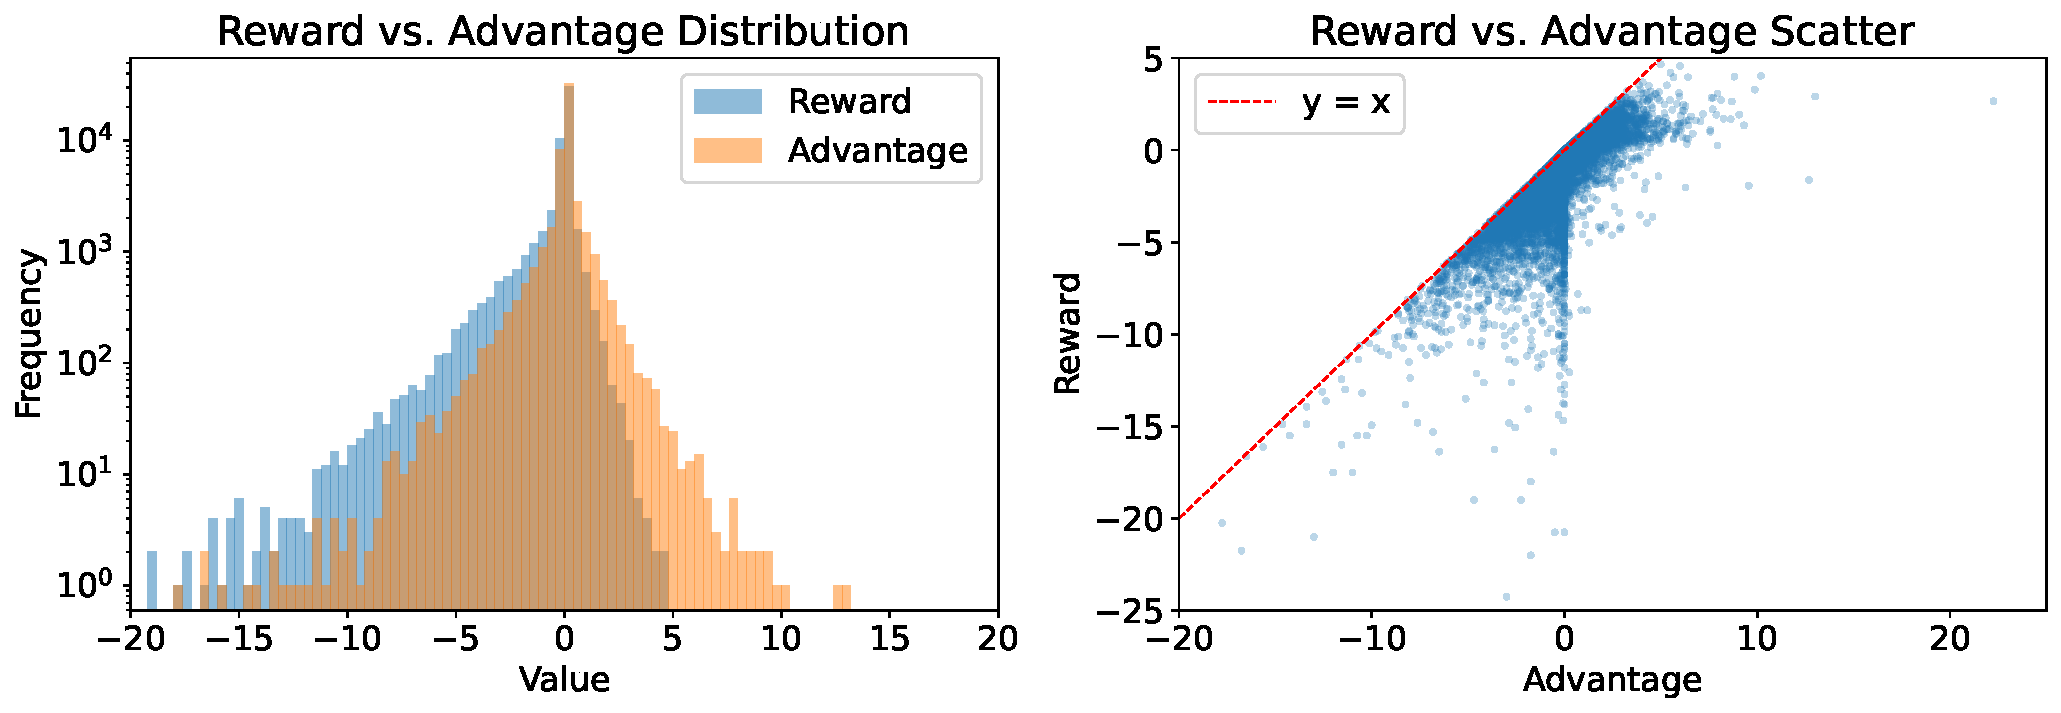
\includegraphics[width=\linewidth]{figures/reward.pdf} 
    \caption{Token-level reward and advantage distributions. \textbf{Left:} The marginal distributions. \textbf{Right:} Per-token scatter plot (x: advantage, y: reward).}
    \label{fig:rewards}
    \vspace{-15pt}
\end{figure}

\paragraph{Advantage vs.\ Reward.} To further understand the effect of \method{}, we examine how the transformation from per-token reward $r_t$ to advantage $a_t = r_t + \mathbb{D}_\mathrm{KL}(\pi_\theta\|\pi_T)$ reshapes the training signal. Specifically, we log all token-level $r_t$ and $a_t$ from the first batch of 64 prompts (approximately 55k tokens) in the Qwen3-1.7B into Qwen3-1.7B-Base setting. Figure~\ref{fig:rewards} (left) shows the frequency distributions. The OPD reward distribution exhibits a pronounced negative long tail, consistent with recent reports~\citep{ko2026scaling} and our discussion in \S~\ref{sec:vopd_value}. The \method{} advantage distribution is visibly shifted rightward with the long tail compressed toward zero, which follows directly from the baseline: since $\mathbb{D}_\mathrm{KL}(\pi_\theta\|\pi_T) \geq 0$, the shift is always non-negative.

We further analyze the token-level effect of this shift in Figure~\ref{fig:rewards} (right), which plots the per-token advantage (x-axis) against reward (y-axis). All points lie on or to the right of $y = x$, confirming that the baseline can only shift rewards positively. Notably, positive-reward tokens are largely unchanged, whereas among tokens with similarly negative rewards, some are dampened almost entirely to zero while others retain advantages close to their original values. This follows directly from the baseline's definition: because the subtracted quantity is the token-level KL divergence at context $c_t$, tokens at high-KL contexts receive a large positive shift that absorbs most of the negative reward, while tokens at low-KL contexts are left nearly intact.

This selectivity has a natural interpretation. A large negative reward arises when the student assigns high probability to a token the teacher considers unlikely. Suppressing this token is likely to shift its mass toward the student's other high-probability candidates. In low-KL contexts, the teacher's density for these alternative tokens is also likely to be high, yielding an informative gradient with minimal influence from \method{}. In high-KL contexts, however, these tokens may be less probable for the teacher, resulting in a harmful gradient that can be mitigated by the high baseline from \method{}. This is consistent with Eq.~\eqref{eq:variance-reduction}, where variance reduction scales with $\mathbb{D}_\mathrm{KL}(\pi_\theta\|\pi_T)^2$, largest at exactly the contexts where updates are least informative. Prior work has identified these high-mismatch tokens as the dominant source of gradient instability in OPD~\citep{li2026rethinkingopd}, and the fact that \method{}'s selective suppression improves rather than degrades accuracy (Table~\ref{tab:math-results}) confirms that what is removed is noise rather than signal---an effect that simple gradient clipping cannot replicate.

\paragraph{Hyperparameter Sensitivity.}
\label{sec:exp_ablation}
We ablate the top-$k$ hyperparameter in \method{}$_\text{top-$k$}$ using the Qwen3-1.7B into Qwen3-1.7B-Base setting. Figure~\ref{fig:ablation} (left) shows that average accuracy is stable across $k \in \{5, 20, 50, 100\}$ and the full-vocabulary baseline, with all values substantially outperforming OPD, which is interpretable as the $k{=}0$ case where no baseline is used. The key finding is that any nonzero $k$ suffices: even the coarsest approximation at $k{=}5$ provides enough variance reduction to stabilize training. Further detailed results are reported in Table~\ref{tab:appendix-math-results} (bottom). Figure~\ref{fig:ablation} (right) plots the mean squared error of the top-$k$ KL estimate relative to the full-vocabulary KL baseline; for base OPD, this equals the squared full-vocabulary KL itself, since no baseline is subtracted. The approximation error is low across all tested values of $k$ and decreases monotonically, dropping to near zero beyond $k{=}20$. Notably, the $k{=}5$ estimate carries non-trivial approximation error yet still matches the accuracy of the full-vocabulary baseline, suggesting that a coarse approximation of the value function is sufficient for stable training, even without a precise estimate.

\begin{figure}[t]
    \centering
    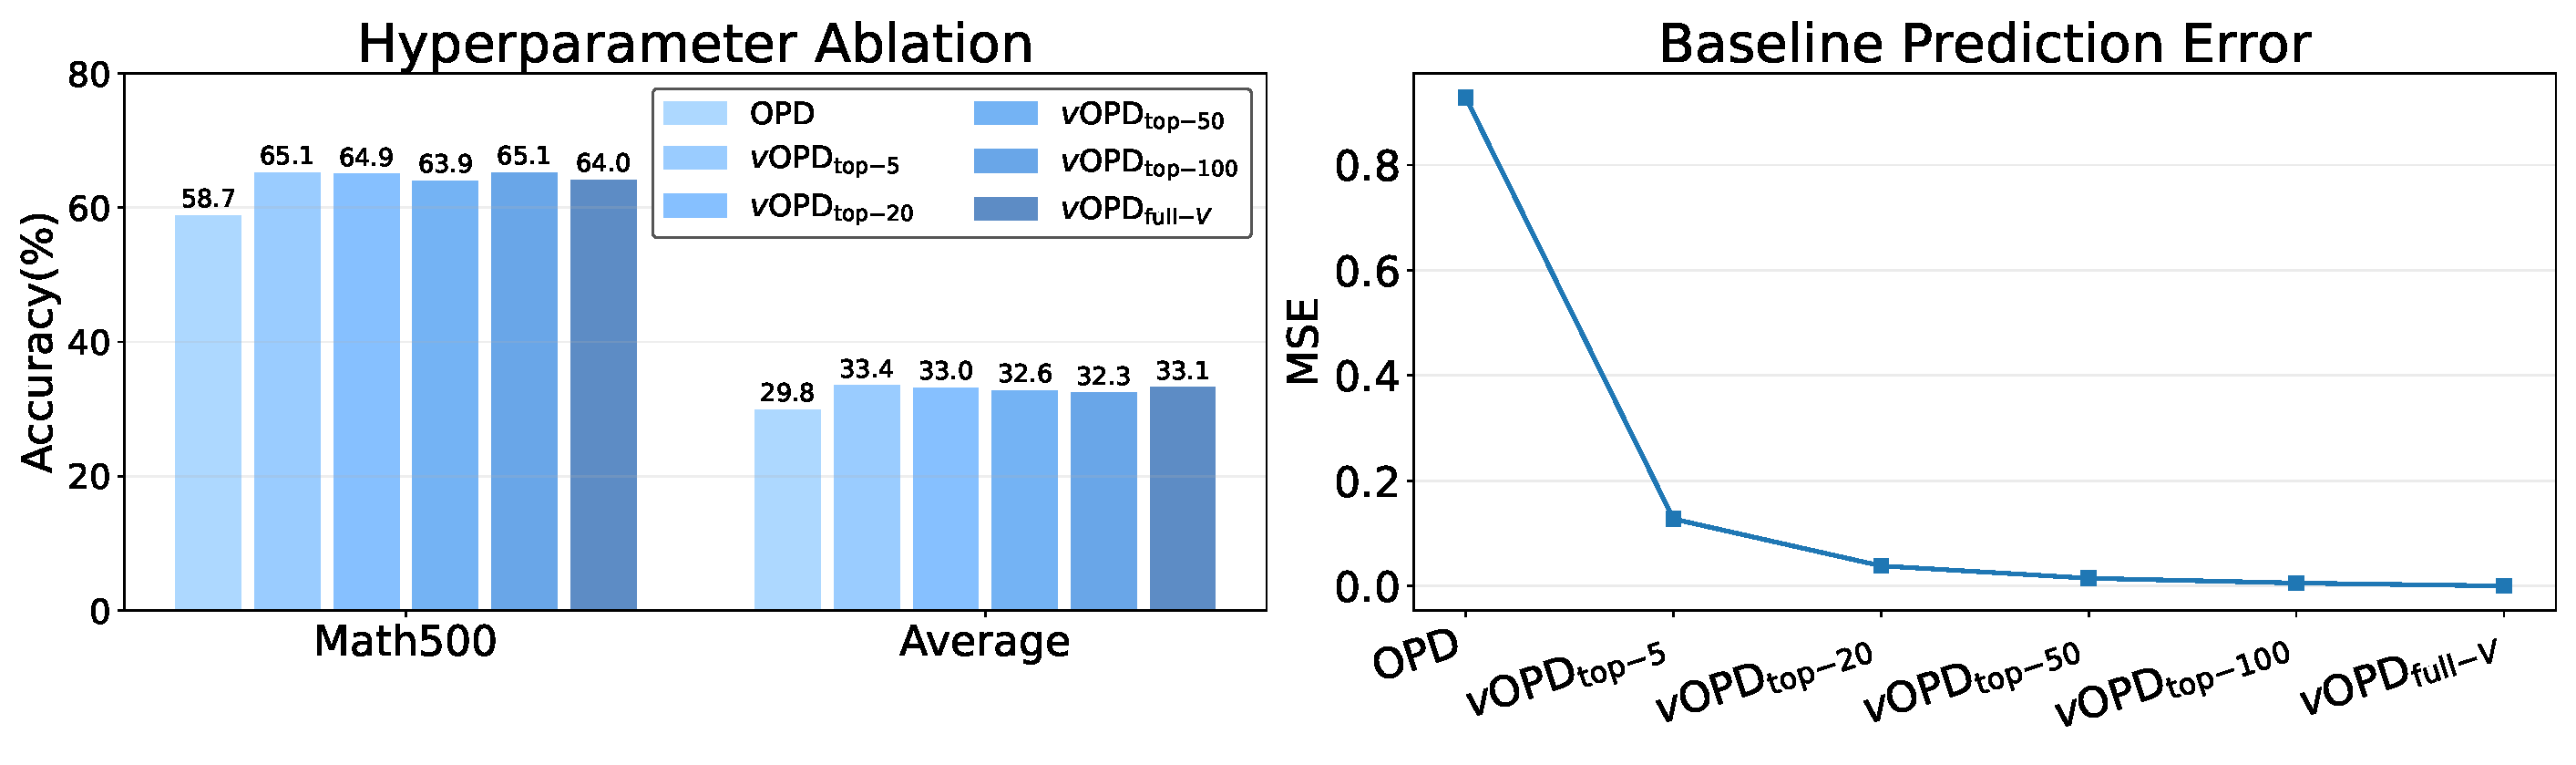
\includegraphics[width=\linewidth]{figures/full_plot_square.pdf} 
    \caption{\textbf{Left:} Average accuracy for various $k$ on \method{}$_\text{top-$k$}$. \textbf{Right:} Mean squared error of the top-$k$ KL baseline relative to the full-vocabulary KL.}
    \label{fig:ablation}
\end{figure}

\paragraph{Wall-Clock Time.}
\begin{figure}
    \centering
    \vspace{-1.0em}
    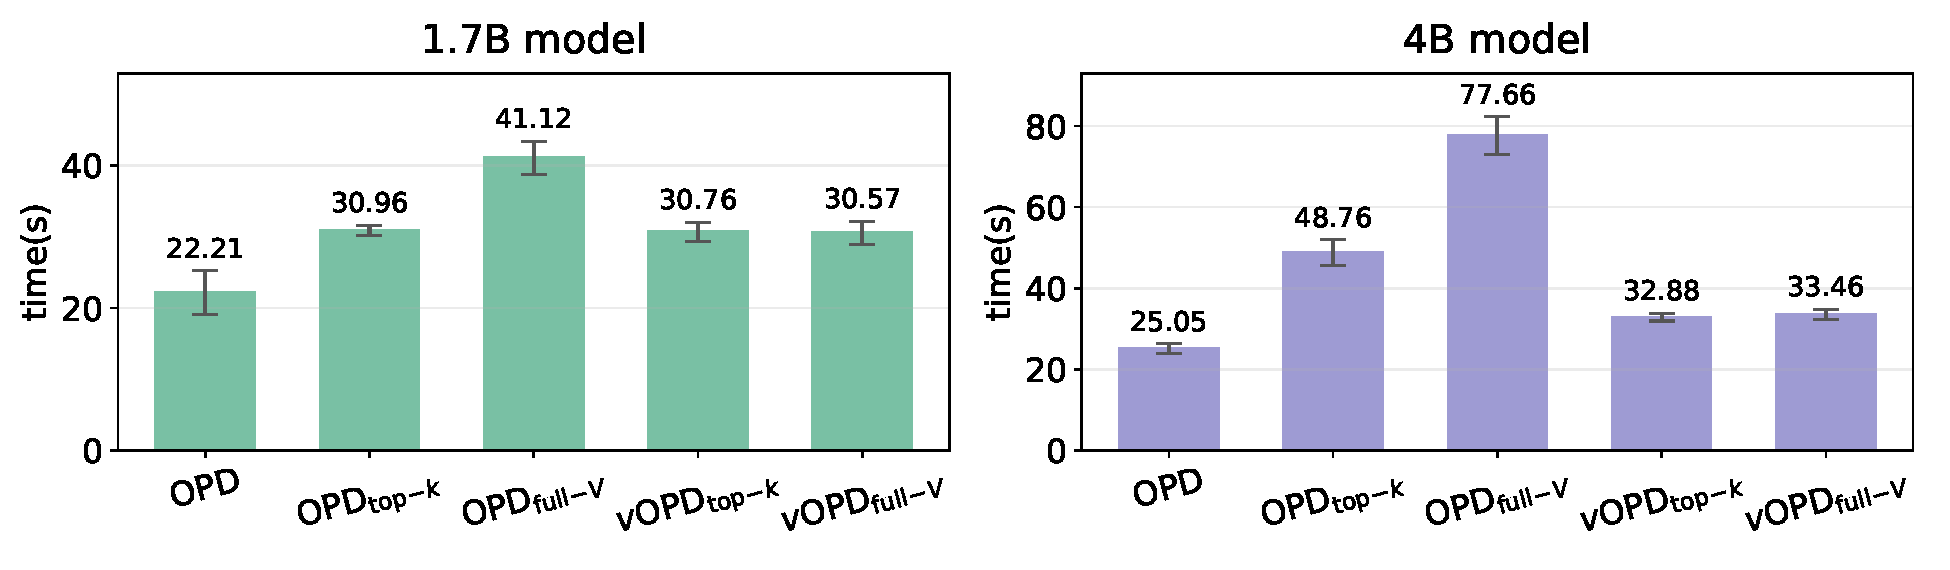
\includegraphics[width=\linewidth]{figures/time.pdf}
    \caption{Per-step wall-clock time for OPD variants at 1.7B and 4B scale.  The error bars denote variance.}
    \label{fig:time}
    \vspace{-1.0em}
\end{figure}
We compare per-step wall-clock time across all five methods at Qwen3-1.7B and 4B scales using a single NVIDIA H200 GPU in Figure~\ref{fig:time}. At 1.7B, base OPD is the fastest, followed by \method{}$_\text{top-$k$}$, \method{}$_\text{full-V}$, and $\text{OPD}_\text{top-$k$}$, which cluster at a modest overhead; $\text{OPD}_\text{full-V}$ is the most expensive due to its full-vocabulary backward pass. At 4B, the gaps widen: $\text{OPD}_\text{top-$k$}$ becomes considerably more expensive compared to both \method{} variants, and \method{}$_\text{top-$k$}$ pulls slightly ahead of \method{}$_\text{full-V}$ in speed, while the overall ordering remains the same. Combined with the results in Table~\ref{tab:math-results}, \method{}$_\text{top-$k$}$ offers the best accuracy-to-compute tradeoff among all compared methods, and the widening gap at 4B scale highlights the scalability advantage of \method{}.

\vspace{-1em}
\begin{wrapfigure}[10]{r}{0.45\linewidth}
    \vspace{-2.0em}
    \centering
    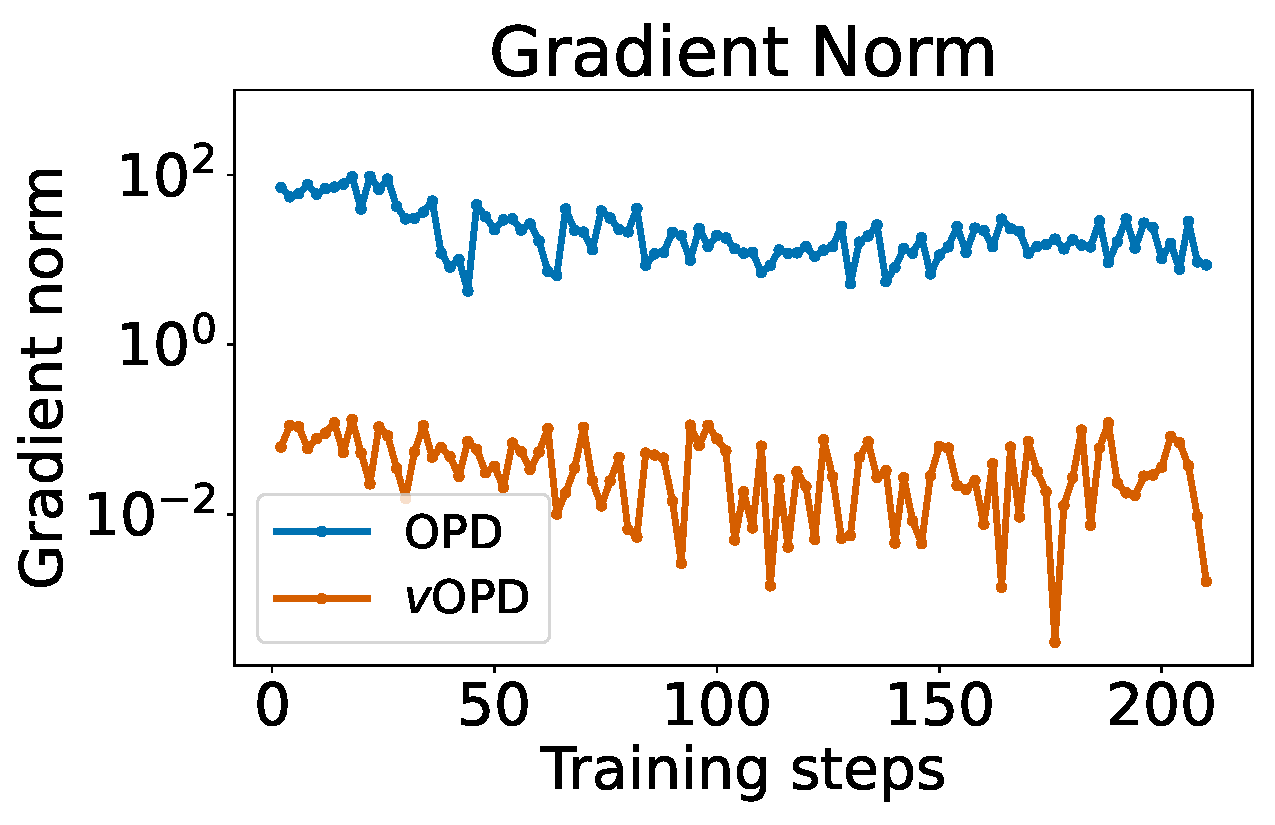
\includegraphics[width=\linewidth]{figures/grad_norm.pdf}
    \caption{Gradient norm in training.}
    \label{fig:grad_norm}
\end{wrapfigure}
\vspace{1em}
\paragraph{Gradient Norm.} To further understand the empirical stabilization effect, we plot gradient norms throughout training for OPD and \method{}$_\text{full-V}$ in the Qwen3-1.7B setting in Figure~\ref{fig:grad_norm}. Notably, \method{} maintains gradient norms 1--2 orders of magnitude lower than base OPD. Despite the substantially smaller gradients, \method{} trains stably and reaches higher accuracy (Table~\ref{tab:math-results}), confirming that the large gradients in base OPD are dominated by variance rather than useful signal, and that \method{} successfully suppresses this instability.

\subsection{Scientific Reasoning Results}
\label{sec:exp-sci}
\begin{wraptable}{r}{0.45\textwidth}
\vspace{-1.25em}
\centering
\caption{Ablation results on scientific reasoning benchmarks. Best performance is \textbf{bolded}, and second best performance is \underline{underlined}.}
\label{tab:science-ablation}
\small
\setlength{\tabcolsep}{5pt}
\begin{tabular}{l|cc}
\toprule
\textbf{Method} & \textbf{SciKnowEval} & \textbf{GPQA-D} \\
\midrule
Student
& 26.1 & 20.4 \\
OPD
& 29.3 & 24.7 \\
OPD$_{\text{top-}k}$
& 29.7 & 24.1 \\
OPD$_{\text{full-V}}$
& \textbf{35.1} & \textbf{28.7} \\
\rowcolor{blue!10}
\method{}$_{\text{top-}k}$
& 33.2 & \underline{28.6} \\
\rowcolor{blue!10}
\method{}$_{\text{full-V}}$
& \underline{34.7} & 28.4 \\
\bottomrule
\end{tabular}
\vspace{-1.0em}
\end{wraptable}
Table~\ref{tab:science-ablation} demonstrates that \method{}'s gains generalize beyond mathematics to SciKnowEval (chemistry) and GPQA-Diamond. The overall findings are consistent with the mathematical reasoning results, as $\text{OPD}_\text{full-V}$ and both \method{} variants lead in performance, gaining around +4\% over base OPD on both benchmarks. Similarly, $\text{OPD}_\text{top-$k$}$ shows little gain over base OPD. The consistency of these results with the mathematical reasoning setting supports the view that \method{}'s gains stem from a general, principled control variate mechanism.

\section{Related Work}
\subsection{On-Policy Distillation}
\label{sec:related-opd}
OPD has become an important component of LLM post-training, especially for long Chain-of-Thought reasoning tasks~\citep{wei2022chain}, where dense token-level teacher signals offer a compute-efficient alternative to sparse RLVR rewards. Early works such as GKD~\citep{agarwal2024onpolicy} and MiniLLM~\citep{gu2024minillm} established OPD as an effective alternative to standard distillation. Recent work has popularized token-level Monte Carlo OPD~\citep{lu2025onpolicydistillation}, studied practical recipes~\citep{patino2025opd,li2026rethinkingopd}, and incorporated OPD into large-scale post-training systems~\citep{yang2025qwen3,zeng2026glm,yang2026nemotron2,deepseekai2026deepseekv4}. Despite these successes, OPD remains unstable in practice. Follow-up studies have explored top-$k$ support restrictions~\citep{li2026rethinkingopd}, entropy-aware training~\citep{jin2026entropy}, and prefix-only variants~\citep{zhang2026prefixopd}. Our work complements these efforts by treating OPD instability as an estimator-variance problem and addressing it with an unbiased control variate baseline.
\subsection{Control Variate Baseline for RL}
\label{sec:related-baselines}
The control variate baseline is a core tool in on-policy policy-gradient reinforcement learning. This principle underlies actor-critic methods, advantage estimation, and modern policy-gradient algorithms such as A3C and PPO with GAE~\citep{williams1992simple,sutton1999policygrad,mnih2016asynchronous,schulman2017ppo,schulman2016high}. The same idea remains central in LLM reinforcement learning. Early RLHF pipelines used PPO~\citep{ouyang2022rlhf, schulman2017ppo} with a learned value model to estimate advantages, while recent reasoning-oriented RLVR methods~\citep{lambert2024tulu} often replace the learned critic with a simpler relative baseline. GRPO and RLOO, for example, use rewards from multiple sampled responses to construct a relative baseline, and have become standard recipes for RLVR~\citep{ahmadian2024back,shao2024deepseekmath,guo2025deepseek, yu2025dapo}. Follow-up methods such as SPO explore alternative single-stream baseline estimators~\citep{xu2025spo}. Despite the central role of the baseline in RL, it has not been systematically explored for OPD, even though OPD admits a policy-gradient interpretation~\citep{lu2025onpolicydistillation,ko2026scaling,jin2026entropy}. Our work fills this gap by deriving a closed-form OPD value baseline and using it as an unbiased control variate.

\section{Conclusion, Limitations, and Future Work}
\label{sec:conclusion}
We introduced \method{}, a control variate formulation of On-Policy Distillation that reduces the variance of the single-sample Monte Carlo estimator without changing the original OPD objective. By using the negative reverse KL between the student and the teacher as a detached value baseline, \method{} preserves an unbiased policy-gradient estimator while retaining the single-token backward pass of base OPD. Experiments on reasoning benchmarks spanning mathematics and science show that \method{} improves training stability and performance over base OPD, acting as a principled regularizer on destabilizing negative reward tokens.

Several directions remain open for future work. Experiments in this work are limited to models up to 7B parameters, and validating \method{} at a larger scale is a next step. Wall-clock results reflect our implementation and are not definitive. Future work could aim to optimize \method{}$_\text{top-$k$}$ to be faster than \method{}$_\text{full-V}$. As a distillation method, \method{} requires access to a stronger teacher; extending it to self-distillation settings is an interesting direction. Finally, this work focuses on the token-level KL in OPD, and considering sequence-level KL objectives is another potential extension.

\newpage
\bibliographystyle{plainnat}
\bibliography{neurips}
%%%%%%%%%%%%%%%%%%%%%%%%%%%%%%%%%%%%%%%%%%%%%%%%%%%%%%%%%%%%
\newpage
\appendix

\section{Theoretical Derivations}
\label{app:theory}

This appendix provides derivations omitted from \S~\ref{sec:prelim} and \S~\ref{sec:method}. Following the main sections, we denote the context $c_t=(x,y_{<t})$, and the reward $r_t(c_t,y_t) = \log\pi_T(y_t\mid c_t) - \log\pi_\theta(y_t\mid c_t)$. We use the score-function identity:
\begin{equation}
\label{eq:app-score}
\sum_{v} \pi_\theta(v\mid c_t)\,\nabla_\theta\log\pi_\theta(v\mid c_t)
\;=\; \sum_{v} \nabla_\theta\,\pi_\theta(v\mid c_t)
\;=\; \nabla_\theta \sum_{v} \pi_\theta(v\mid c_t)
\;=\; 0,
\end{equation}
which follows from the log trick $\nabla_\theta\log\pi_\theta(v\mid c_t) = \nabla_\theta\pi_\theta(v\mid c_t)/\pi_\theta(v\mid c_t)$.

\subsection{Unbiasedness of Baseline Subtraction}
\label{app:unbiased}

We show that subtracting an action-independent baseline $b_t(c_t)$ from the per-token reward leaves the policy gradient unbiased~\citep{williams1992simple,sutton1999policygrad}.
Specifically, we show:
\begin{equation}
\label{eq:app-unbiased-claim}
\mathbb{E}_{y_t \sim \pi_\theta(\cdot\mid c_t)}\!\Bigl[
  \bigl(r_t(y_t) - b_t(c_t)\bigr)\,\nabla_\theta\log\pi_\theta(y_t\mid c_t)
\Bigr]
\;=\;
\mathbb{E}_{y_t \sim \pi_\theta(\cdot\mid c_t)}\!\Bigl[
  r_t(y_t)\,\nabla_\theta\log\pi_\theta(y_t\mid c_t)
\Bigr].
\end{equation}

By linearity of expectation, the difference between the two sides equals
\begin{equation}
    \mathbb{E}_{y_t \sim \pi_\theta(\cdot\mid c_t)}\!\Bigl[
  b_t(c_t)\,\nabla_\theta\log\pi_\theta(y_t\mid c_t)
\Bigr]
\;=\;
b_t(c_t)
\sum_{v} \pi_\theta(v\mid c_t)\,\nabla_\theta\log\pi_\theta(v\mid c_t),
\end{equation}
where $b_t(c_t)$ factors out of the expectation because it is independent of $y_t$ by assumption. The score-function identity (Eq.~\eqref{eq:app-score}) gives the remaining sum as zero, so the difference vanishes and Eq.~\eqref{eq:app-unbiased-claim} holds.

\subsection{Variance Reduction and the Optimal Baseline}
\label{app:variance}

We derive the variance-reducing property of baseline subtraction and identify the optimal scalar choice~\citep{greensmith2004variance}. Consider the per-step gradient estimator:
\begin{equation}
    g(b) \;=\; \bigl(r_t(y_t) - b\bigr)\,\nabla_\theta\log\pi_\theta(y_t\mid c_t),
\qquad b \in \mathbb{R}.
\end{equation}
We seek the $b$ minimizing $\mathrm{tr}(\mathrm{Var}[g(b)])$. $\mathbb{E}[g(b)]$ does not depend on $b$ because baseline subtraction is unbiased (\S~\ref{app:unbiased}), so the variance is minimized by minimizing the second moment $\mathbb{E}[\|g(b)\|^2]$. Expanding,
\begin{align}
\mathbb{E}\!\bigl[\|g(b)\|^2\bigr]
&\;=\;
  \mathbb{E}\!\Bigl[
    \bigl(r_t(y_t) - b\bigr)^2\,
    \bigl\|\nabla_\theta\log\pi_\theta(y_t\mid c_t)\bigr\|^2
  \Bigr] \\[4pt]
&\;=\;
  \mathbb{E}\!\Bigl[r_t(y_t)^2\,\bigl\|\nabla_\theta\log\pi_\theta(y_t\mid c_t)\bigr\|^2\Bigr]
  \;-\; 2b\,\mathbb{E}\!\Bigl[r_t(y_t)\,\bigl\|\nabla_\theta\log\pi_\theta(y_t\mid c_t)\bigr\|^2\Bigr] \\
&\quad+\; b^2\,\mathbb{E}\!\Bigl[\bigl\|\nabla_\theta\log\pi_\theta(y_t\mid c_t)\bigr\|^2\Bigr].
\end{align}

This is a convex quadratic in $b$. Setting its derivative to zero yields the
\emph{optimal scalar baseline} $b^\star$:
\begin{equation}
\label{eq:app-optimal-baseline}
b^\star
\;=\;
\frac{
  \mathbb{E}_{y_t \sim \pi_\theta(\cdot\mid c_t)}\!\Bigl[
    r_t(y_t)\,\bigl\|\nabla_\theta\log\pi_\theta(y_t\mid c_t)\bigr\|^2
  \Bigr]
}{
  \mathbb{E}_{y_t \sim \pi_\theta(\cdot\mid c_t)}\!\Bigl[
    \bigl\|\nabla_\theta\log\pi_\theta(y_t\mid c_t)\bigr\|^2
  \Bigr]
}.
\end{equation}
The optimal baseline in Eq.~\eqref{eq:app-optimal-baseline} is a weighted form of
the value function. In practice, the value function itself is used as the baseline,
motivating the choice in \S~\ref{sec:vopd_value}:
\begin{equation}
    b^\star
\;\approx\;
\mathbb{E}_{y_t \sim \pi_\theta(\cdot\mid c_t)}\!\bigl[r_t(y_t)\bigr]
\;=\; V^{\pi_\theta}(c_t).
\end{equation}

\subsection{Variance Reduction of \method{}}
\label{app:variance-derivation}
We now derive Eq.~\eqref{eq:variance-reduction}, the per-step variance reduction
obtained by \method$_\text{full-V}$. Recall the two estimators:
\begin{equation}
g_\text{OPD} =r_t(c_t, y_t)\,\nabla\!\log\pi_\theta(y_t\mid c_t),
\qquad
g_{\text{\method}_{\text{full-V}}} = \bigl(r_t(c_t, y_t) - b_t\bigr)\,\nabla\!\log\pi_\theta(y_t\mid c_t),
\end{equation}
where $b_t = V^{\pi_\theta}(c_t) = -\mathbb{D}_\mathrm{KL}(\pi_\theta(\cdot\mid c_t)\,\|\,\pi_T(\cdot\mid c_t))$. We want to show:
\begin{equation}
\label{eq:app-vopd-variance-claim}
\mathrm{tr}\!\bigl(\mathrm{Var}[g_\text{OPD}]\bigr) - \mathrm{tr}\!\bigl(\mathrm{Var}[g_{\text{\textnormal{\method}}_{\text{full-V}}}]\bigr)
\;\approx\;
\mathbb{D}_\mathrm{KL}\!\bigl(\pi_\theta(\cdot\mid c_t)\,\big\|\,\pi_T(\cdot\mid c_t)\bigr)^{2}
\;\cdot\;
\mathbb{E}\!\bigl[\|\nabla\!\log\pi(y_t\mid c_t)\|^2\bigr].
\end{equation}
We start from the second-moment expansion of \S~\ref{app:variance}. Since both
estimators share the same expectation (by \S~\ref{app:unbiased}), the variance
difference equals the difference of second moments:
\begin{align*}
\mathrm{tr}\!\bigl(\mathrm{Var}[g_\text{OPD}]\bigr) - \mathrm{tr}\!\bigl(\mathrm{Var}[g_{\text{\method}_{\text{full-V}}}]\bigr)
&\;=\; \mathbb{E}\!\bigl[r_t^2\,\|\nabla\!\log\pi_\theta(y_t|c_t)\|^2\bigr]
- \mathbb{E}\!\bigl[(r_t - b_t)^2\,\|\nabla\!\log\pi_\theta(y_t|c_t)\|^2\bigr] \\
&\;=\; 2b_t\,\mathbb{E}\!\bigl[r_t\,\|\nabla\!\log\pi_\theta(y_t|c_t)\|^2\bigr]
- b_t^2\,\mathbb{E}\!\bigl[\|\nabla\!\log\pi_\theta(y_t|c_t)\|^2\bigr].
\end{align*}
Under a weak-correlation approximation $\mathbb{E}[r_t\,\|\nabla\!\log\pi_\theta(y_t|c_t)\|^2] \approx b_t\,\mathbb{E}[\|\nabla\!\log\pi_\theta(y_t|c_t)\|^2]$, this yields:
\begin{equation}
\mathrm{tr}\!\bigl(\mathrm{Var}[g_\text{OPD}]\bigr) - \mathrm{tr}\!\bigl(\mathrm{Var}[g_{\text{\method}_{\text{full-V}}}]\bigr)
\;\approx\;
b_t^2\,\mathbb{E}\!\bigl[\|\nabla\!\log\pi_\theta(y_t|c_t)\|^2\bigr].
\end{equation}
Substituting $b_t^2 = \mathbb{D}_\mathrm{KL}(\pi_\theta\|\pi_T)^2$ recovers Eq.~\eqref{eq:app-vopd-variance-claim}.

\paragraph{Weak-correlation approximation.}
We discuss why a weak-correlation assumption is reasonable in the OPD setting. Because $y_t$ is sampled from $\pi_\theta$, sampled tokens naturally lie in the high-probability region, so $\log\pi_\theta(y_t\mid c_t)$ varies in a narrow band and
$\|\nabla\!\log\pi\|^2$, a function of $\pi_\theta$ at $y_t$, can inherit this concentration. In contrast, the variation in $r_t = \log\pi_T(y_t\mid c_t) - \log\pi_\theta(y_t\mid c_t)$ is primarily driven by the teacher term, which has no structural dependence on $\pi_\theta(y_t \mid c_t)$. Figure~\ref{fig:logp-scatter} confirms this empirically, showing scatter plots from the same data used in \S~\ref{sec:exp-further}: $\log\pi_\theta(y_t)$ concentrates near zero with weak correlation to $r_t$, while $\log\pi_T(y_t \mid c_t)$ spans a wider range and exhibits a clear correlation with $r_t$. This is also consistent with the analysis in \S~\ref{sec:exp-further} and recent long-tail negative reward structure report~\citep{ko2026scaling}: since $\log\pi_\theta(y_t \mid c_t)$ stays close to zero, $r_t$ cannot spike in the positive direction, but can extend into large negative values whenever $\log\pi_T(y_t \mid c_t)$ drops---making the teacher term the dominant driver of variation in $r_t$.

\begin{figure}[!h]
    \centering
    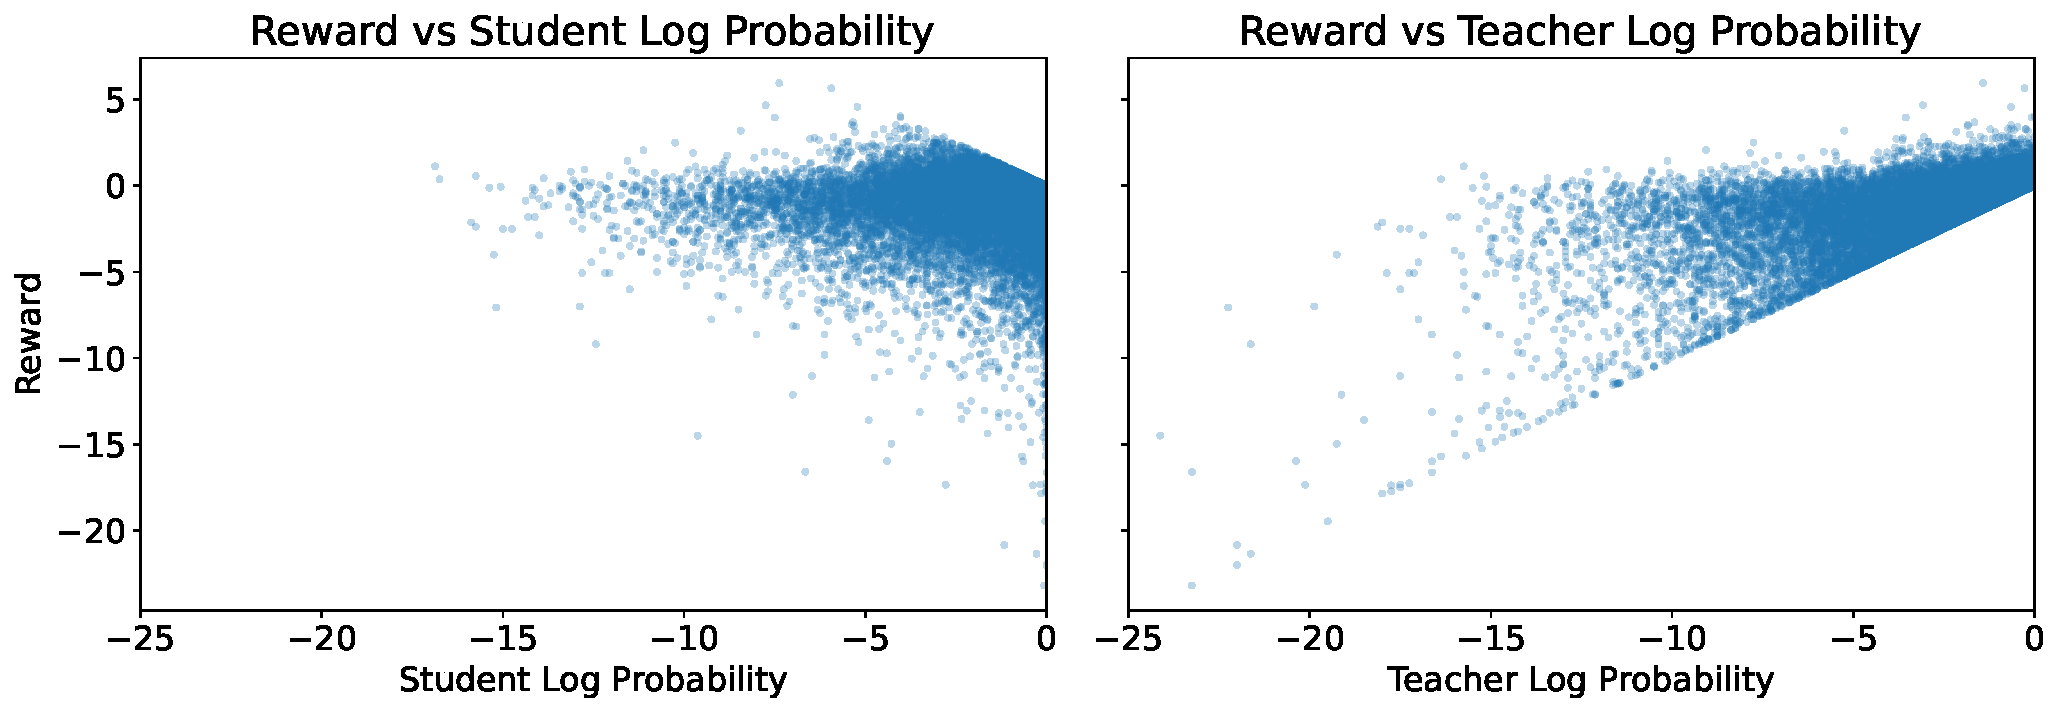
\includegraphics[width=0.8\linewidth]{figures/reward_vs_logp_combined.pdf}
    \caption{Scatter plot. \textbf{Left:} student log probability ($x$) vs.\ reward ($y$).
    \textbf{Right:} teacher log probability ($x$) vs.\ reward ($y$).}
    \label{fig:logp-scatter}
    \vspace{-15pt}
\end{figure}

\section{Experiment Settings}
\label{app:exp_settings}
This section details the experimental settings from \S~\ref{sec:exp_setup}. All experiments were conducted on a single NVIDIA H200 NVL or A100 NVL GPU, paired with an Intel(R) Xeon(R) Gold 6530 or Gold 6230 CPU @ 2.10GHz, respectively. All training runs took between 2h (1.7B on A100) and 6h (7B on H200).

\subsection{Training Settings}
Table~\ref{tab:hyperparameters_all} summarizes the hyperparameters for training and evaluation.
Following recent work demonstrating that the maximum response length in OPD need not be excessively long (2--3K tokens suffice), we set the maximum response length to 2048~\citep{zhang2026prefixopd, li2026rethinkingopd}. Following recent work on OPD, we set the student sampling temperature to 1.0~\citep{li2026rethinkingopd,ko2026scaling}. We adopt parameter-efficient training via LoRA~\citep{hu2022lora}.
Our implementation builds on \texttt{TRL}'s MiniLLM\footnote{\url{https://huggingface.co/docs/trl/main/minillm}} implementation~\citep{vonwerra2020trl,gu2024minillm}. When using Qwen as the teacher model, we disable its extended thinking mode. For scientific reasoning, which comprises 1,890 train samples from the chemistry subset of SciKnowEval~\citep{feng2024sciknoweval}, we extend training to a maximum of 10 epochs.

For evaluation, following the official guidelines for Qwen3 and Olmo-3 \cite{yang2025qwen3, olmo2025olmo}, we set the sampling temperature to 0.6 and top-p sampling to 0.9. We use \texttt{vLLM} for accelerated inference~\citep{kwon2023efficient}.


\begin{table}[!h]
\centering
\caption{Training and Evaluation Settings}
\label{tab:hyperparameters_all}
\small
\setlength{\tabcolsep}{4pt}
\begin{tabular}{l|c|c||l|c|c}
\toprule
\textbf{Hyperparameter} & \textbf{Train} & \textbf{Eval}
& \textbf{Hyperparameter} & \textbf{Train} & \textbf{Eval} \\
\midrule
Prompt length   & 1024 & 1024
& Response length & 2048 & 4096 \\
Rollout temperature     & 1.0 & 0.6
& Top-$p$ sampling        & 1.0 & 0.9 \\
Batch size              & 64 & --
& Optimizer              & AdamW & -- \\
Learning rate           & 1e-5 (Qwen3), 2e-5 (Olmo-3) & --
& LoRA rank               & 64 & -- \\
Epochs                  & 1 (math), 10 (science) & --
& LoRA $\alpha$          & 128 & -- \\
Engine                  & \texttt{TRL} & \texttt{vLLM}
& Precision               & \texttt{bfloat16} & \texttt{bfloat16} \\
\bottomrule
\end{tabular}
\end{table}

\subsection{Prompts}
We use the following prompts for mathematical and scientific reasoning throughout training and evaluation, following the official prompts~\citep{yang2025qwen3}.
\begin{tcolorbox}[
    colback=gray!5,
    colframe=gray!50,
    title=\textbf{Math Reasoning Prompt Template},
    fonttitle=\bfseries,
    boxrule=0.5pt,
    arc=2pt,
]
\small
\texttt{\{problem\}}\textbackslash n\textbackslash nPlease reason step by step, and put your final answer within \textbackslash \textbackslash boxed\{\}.

\vspace{0.5em}

\end{tcolorbox}


\begin{tcolorbox}[
    colback=gray!5,
    colframe=gray!50,
    title=\textbf{Scientific Reasoning Prompt Template},
    fonttitle=\bfseries,
    boxrule=0.5pt,
    arc=2pt,
]
\small
\texttt{\{problem\}}\textbackslash n\textbackslash nReturn only one JSON object with the key "answer". The value must be exactly one choice letter, for example: \{"answer": "C"\}.
\end{tcolorbox}

\section{Extended Experiment Results}
Table~\ref{tab:appendix-math-results} presents the extended results. Specifically, it reports: (i) the accuracy of the teacher models used in our experiments; (ii) the results of distilling Qwen3-1.7B into Qwen3-0.6B-Base, from \S~\ref{sec:exp-math}; and (iii) comprehensive benchmark results for the hyperparameter ablations in Figure~\ref{fig:ablation}.

\begin{table}[!h]
\centering
\caption{Additional mathematical reasoning benchmark results. Best performance is \textbf{bolded}, and second best performance is \underline{underlined}.}
\label{tab:appendix-math-results}
\resizebox{\textwidth}{!}{%
\begin{tabular}{l|cc|cc|cc|cc|c}
\toprule
& \multicolumn{2}{c|}{\textbf{MATH500}} 
& \multicolumn{2}{c|}{\textbf{MINERVA}} 
& \multicolumn{2}{c|}{\textbf{AMC23}} 
& \multicolumn{2}{c|}{\textbf{AIME24/25}} 
& \\
\cmidrule(lr){2-3} 
\cmidrule(lr){4-5} 
\cmidrule(lr){6-7} 
\cmidrule(lr){8-9}
\textbf{Method} 
& Avg@8 & Pass@8 
& Avg@8 & Pass@8 
& Avg@32 & Pass@32 
& Avg@32 & Pass@32 
& \textbf{Avg.} \\
\midrule
\multicolumn{10}{c}{\textit{Teacher Performance}} \\
\midrule
Qwen3-1.7B 
& 73.0 & 90.8 & 28.6 & 42.6 & 44.8 & 85.0 & 14.4 & 35.0 & 40.2 \\
Qwen3-4B 
& 83.5 & 93.8 & 43.9 & 49.6 & 65.9 & 95.0 & 20.2 & 51.7 & 53.4 \\
Olmo-3-7B-Think 
& 87.2 & 95.4 & 39.2 & 52.2 & 70.0 & 97.5 & 37.2 & 68.3 & 58.4 \\
\midrule
\multicolumn{10}{c}{\textit{Qwen3-1.7B $\rightarrow$ Qwen3-0.6B-Base}} \\
\midrule
Student 
& 30.9 & 66.8 & 5.6 & 21.7 & 12.3 & 60.0 & 0.4 & 6.7 & 12.3 \\
OPD 
& 41.4 & \underline{73.0} & 8.1 & 26.1 & 19.3 & \textbf{80.0} & 1.1 & \underline{13.3} & 17.5 \\
OPD$_{\text{top-}k}$ 
& 43.7 & 72.0 & 12.7 & \textbf{32.4} & \underline{21.8} & 65.0 & \textbf{1.5} & \textbf{13.4} & 19.9 \\
OPD$_{\text{full-V}}$
& \textbf{47.3} & 72.0 & 12.8 & 29.4 & 20.7 & 65.0 & \underline{1.4} & \underline{13.3} & \underline{20.6} \\
\rowcolor{blue!10}
\method{}$_{\text{top-}k}$ 
& 44.4 & 71.0 & \underline{13.7} & 29.0 & 20.9 & \underline{67.5} & 0.9 & 10.0 & 20.0 \\
\rowcolor{blue!10}
\method{}$_{\text{full-V}}$
& \underline{46.5} & \textbf{73.2} & \textbf{14.3} & \underline{32.0} & \textbf{22.3} & \underline{67.5} & \underline{1.4} & 10.0 & \textbf{21.1} \\
\midrule
\multicolumn{10}{c}{\textit{Qwen3-1.7B $\rightarrow$ Qwen3-1.7B-Base (Ablation)}} \\
\midrule
OPD 
& 58.7 & 82.6 & 22.2 & 40.8 & 33.4 & 77.5 & 4.8 & \textbf{28.3} & 29.8 \\
\method{}$_{\text{top-}5}$ 
& \textbf{65.1} & 83.8 & \underline{26.0} & \underline{45.2} & \underline{35.6} & \underline{85.0} & \textbf{6.7} & \underline{26.7} & \textbf{33.4} \\
\method{}$_{\text{top-}20}$ 
& \underline{64.9} & \textbf{84.8} & 25.2 & 44.5 & \textbf{36.1} & 82.5 & 5.6 & \underline{26.7} & 33.0 \\
\method{}$_{\text{top-}50}$ 
& 63.9 & \underline{84.6} & 25.6 & 44.1 & 35.0 & \textbf{87.5} & 6.1 & 23.3 & 32.6 \\
\method{}$_{\text{top-}100}$ 
& \textbf{65.1} & 76.4 & 25.7 & 32.0 & 33.4 & 75.0 & 5.2 & \underline{26.7} & 32.3 \\
\method{}$_{\text{full-V}}$ 
& 64.0 & \underline{84.6} & \textbf{26.2} & \textbf{48.9} & \textbf{36.1} & 80.0 & \underline{6.2} & 25.0 & \underline{33.1} \\
\bottomrule
\end{tabular}%
}
\end{table}

\end{document}